\renewcommand{\stage}{2. Estimating a partially observed model}

\begin{frame}{2. Differentiable particle filters}
{\Large Automatic Differentiation for Inference\\on Partially Observed Markov Process Models}\gap
Joint work: Kevin Tan, A. J. Abkemeier, Kunyang He,\\Giles Hooker, Edward L. Ionides.
\gap JRSS-B, revise and resubmit.\par
\vspace{6mm}
How do we fit a model when we can simulate its states but cannot observe them?
\end{frame}

\begin{frame}{Monthly cholera deaths in Dhaka, 1891--1940}
\begin{center}\begin{tikzpicture}
\begin{axis}[width=.88\textwidth,height=4.3cm,xlabel=Year,ylabel={Deaths per month},xmin=1890,xmax=1942,xtick={1891,1900,1910,1920,1930,1940},scaled x ticks=false,xticklabel style={/pgf/number format/1000 sep={}},ymin=0,axis lines=left, tick label style={font=\small},legend style={draw=none,font=\small},legend pos=north east]
\addplot[blue,thick] table[x=time,y=deaths,col sep=comma]{figures/dhaka-monthly.csv};
\addlegendentry{Recorded deaths}
\end{axis}\end{tikzpicture}\end{center}
\uncover<2->{What can deaths tell us about infections and recoveries?}
\src{King et al. (2008). Data from PyPOMP.}
\end{frame}

\begin{frame}{The Dhaka cholera model}
\begin{center}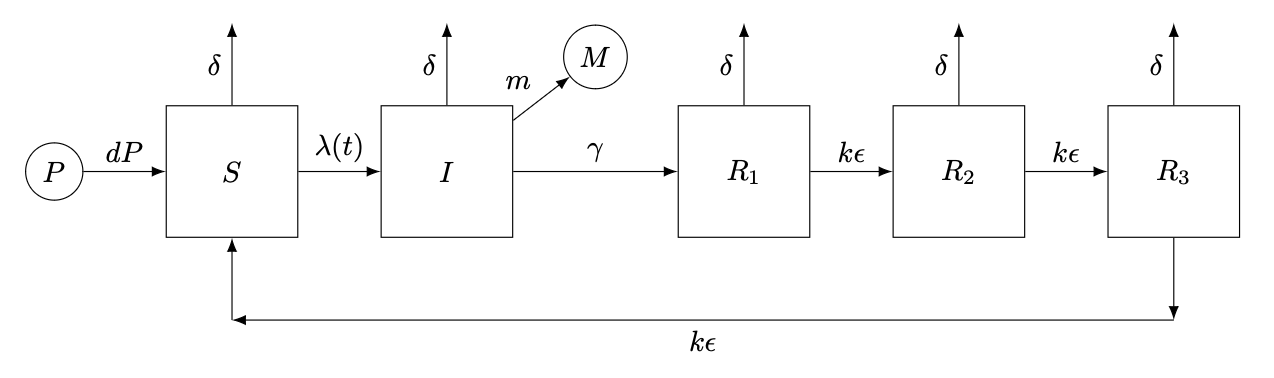
\includegraphics[width=.96\linewidth,height=3.25cm,keepaspectratio]{cholera.png}\end{center}
\textcolor{blue}{Hidden $X_n$}\quad Susceptible, infected and immune populations, plus modeled deaths.
\pause\gap
\textcolor{green}{Observed $y_n$}\quad Monthly deaths, measured with error.
\pause\gap
Which recovery rate $\gamma$ best fits these 600 monthly death counts?
\src{$I\to R_1$ denotes recovery. $R_1,R_2,R_3$ are stages of immunity. King et al. (2008).}
\end{frame}

\begin{frame}{Updating the state distribution}
For fixed parameters $\theta$, $b_n$ is the distribution of hidden states given deaths observed through month $n$.
\[
 b_n(dx)=\frac{1}{L_n}\,
 \underbrace{\textcolor{green}{g_\theta(y_n\mid x)}}_{\text{measurement}}
 \int
 \underbrace{\textcolor{blue}{P_\theta(dx\mid z)}}_{\text{process}}\,
 \underbrace{\textcolor{pink}{b_{n-1}(dz)}}_{\text{last month's filter}} .
\]
\pause We average predictions over last month's state distribution, then weight them by the density of observed deaths.
\pause\gap
$L_n=p_\theta(y_n\mid y_{1:n-1})$ is the predictive density. The likelihood is $\prod_n L_n$.
\end{frame}

% Illustrative counts and measurement densities, not a fitted Dhaka trajectory.
\begin{frame}{Predicting next month's populations}
A particle gives possible counts of susceptible ($S$), infected ($I$) and immune ($R$) people.
\begin{center}\begin{tikzpicture}[x=1cm,y=1cm,font=\small]
\path[use as bounding box] (0,-.1) rectangle (12.4,4.35);
\node at (2.4,4.1) {Last month's particles};
\node at (8.25,4.1) {Predicted populations};
\foreach \x/\label/\col in {1.25/S/blue,2.35/I/pink,3.45/R/green,7.15/S/blue,8.25/I/pink,9.35/R/green}{
\node[text=\col] at (\x,3.65) {$\label$};}
\node[align=center] at (11.3,3.7) {Modeled\\deaths};
\foreach \j/\y/\s/\i/\r/\ss/\ii/\rr/\d in {
1/3.1/900/60/40/880/65/50/5,
2/2.5/850/90/60/820/95/75/10,
3/1.9/800/120/80/760/130/95/15,
4/1.3/870/80/50/845/85/62/8,
5/.7/920/50/30/905/45/47/3}{
\node[left] at (.55,\y) {$\j$};
\foreach \x/\v/\col in {1.25/\s/blue,2.35/\i/pink,3.45/\r/green}{
\node[fill=\col!10,minimum width=10mm,minimum height=5mm] at (\x,\y){\v};}
\begin{scope}[visible on=<2->]
\draw[arr,black!45] (4.2,\y)--(6.3,\y);
\foreach \x/\v/\col in {7.15/\ss/blue,8.25/\ii/pink,9.35/\rr/green}{
\node[fill=\col!10,minimum width=10mm,minimum height=5mm] at (\x,\y){\v};}
\node at (11.1,\y){\d};
\end{scope}}
\node[align=center] at (5.25,3.8) {Simulate\\one month};
\end{tikzpicture}\end{center}
\uncover<2->{\[\widetilde X_n^j\sim P_\theta(\cdot\mid X_{n-1}^j),\qquad j=1,\ldots,J.\]}
\src{Illustrative counts, $J=5$ particles. $R$ combines the immunity stages. The full state also tracks modeled deaths.}
\end{frame}

\begin{frame}{Weighting particles by observed deaths}
Observed this month: $y_n=12$ deaths.
\begin{center}\begin{tikzpicture}[x=1cm,y=.9cm,font=\small]
\path[use as bounding box] (0,-.6) rectangle (12.7,3.9);
\foreach \x/\label/\col in {1/S/blue,2/I/pink,3/R/green}{\node[text=\col] at (\x,3.5){$\label$};}
\node[align=center] at (4.4,3.5){Modeled\\deaths};
\foreach \j/\y/\s/\i/\r/\d in {
1/2.9/880/65/50/5,
2/2.3/820/95/75/10,
3/1.7/760/130/95/15,
4/1.1/845/85/62/8,
5/.5/905/45/47/3}{
\node[left] at (.35,\y){$\j$};
\foreach \x/\v/\col in {1/\s/blue,2/\i/pink,3/\r/green}{
\node[fill=\col!10,minimum width=9mm,minimum height=5mm] at (\x,\y){\v};}
\node at (4.4,\y){\d};}
\begin{scope}[visible on=<2->]
\draw[arr,thick] (5.15,1.8)--(7.65,1.8);
\node[align=center] at (6.4,2.85){Measurement\\density, then\\normalize};
\node at (6.4,1.15){$g_\theta(y_n\mid\widetilde X_n^j)$};
\draw[arr] (8.1,.5)--(12.5,.5);
\node at (10.3,-.4){Particle};
\draw[arr] (8.1,.5)--(8.1,3.4);
\node at (10.3,3.7){Normalized weight};
\foreach \x/\y/\j in {8.6/1.05/1,9.45/2.8/2,10.3/2.3/3,11.15/1.65/4,12/.85/5}{
\fill[blue!65] (\x-.23,.5) rectangle (\x+.23,\y);
\draw (\x,.5)--(\x,.42);\node[below] at (\x,.4){$\j$};}
\end{scope}
\end{tikzpicture}\end{center}
\vspace{-2mm}
\uncover<2->{\[
\overline g_n^j=\frac{g_n^j}{\sum_m g_n^m},\qquad
\underbrace{\sum_j\overline g_n^j\delta_{\widetilde X_n^j}}_{\text{updated state distribution}}\approx b_n,\qquad
\underbrace{\widehat L_n=\frac1J\sum_jg_n^j}_{\text{likelihood increment}}.
\]}
\src{Illustrative compartment counts and schematic weights. $g_n^j=g_\theta(y_n\mid\widetilde X_n^j)$; $\delta_x$ is a point mass.}
\end{frame}

\begin{frame}{Resampling particles}
\begin{center}\begin{tikzpicture}[x=1cm,y=1cm,font=\small]
\path[use as bounding box] (0,0) rectangle (12.4,4.6);
\foreach \j/\y/\r/\sir in {
1/3.5/.135/{(880,65,50)},2/2.8/.28/{(820,95,75)},3/2.1/.248/{(760,130,95)},4/1.4/.198/{(845,85,62)},5/.7/.108/{(905,45,47)}}{
\fill[blue] (4.3,\y) circle(\r);
\node at (2,\y){$\sir$};\node[left] at (.55,\y){$\j$};}
\foreach \j/\y/\py/\sir in {
1/3.5/2.8/{(820,95,75)},2/2.8/2.1/{(760,130,95)},3/2.1/2.1/{(760,130,95)},4/1.4/2.1/{(760,130,95)},5/.7/1.4/{(845,85,62)}}{
\begin{scope}[visible on=<2->]
\fill[blue] (8.3,\y) circle(3pt);
\draw[arr,blue!55] (4.6,\py)--(8.1,\y);
\node at (10.2,\y){$\sir$};
\end{scope}}
\node at (2.3,4.25){Weighted $(S,I,R)$ candidates};
\node at (9.8,4.25){Equally weighted copies};
\end{tikzpicture}\end{center}
\uncover<2->{\[A_n^{1:5}=(2,3,3,3,4),\qquad X_n^j=\widetilde X_n^{A_n^j}.\]}
\uncover<2->{$A_n^j$ is the parent selected for copy $j$, with probability $\overline g_n^{A_n^j}$.}
\src{One possible resampling draw. Circle area is proportional to weight. Each copy carries the full state, including modeled deaths.}
\end{frame}

% Shared axes keep the fixed-seed PF and reweighted likelihood pictures aligned.
\newcommand{\likelihoodaxes}{%
\path[use as bounding box] (0,-.7) rectangle (12.4,4.7);
\draw[arr] (1.5,.6)--(11.8,.6) node[right]{$\theta$};
\draw[arr] (1.5,.6)--(1.5,4.15);
\node[rotate=90] at (.55,2.4){Log likelihood};
\draw (4,.52)--(4,.68);\node[below] at (4,.48){$\phi$};
\draw[black!35,dashed] (4,.7)--(4,2.1);
}
\newcommand{\pfleftcurve}{%
\draw[blue,very thick,domain=1.8:5.4,samples=35] plot (\x,{2.1+.17*(\x-4)+.025*(\x-4)^2});
}
\newcommand{\pfrightcurve}{%
\draw[blue,very thick,domain=5.4:11.2,samples=40] plot (\x,{3.3+.2*(\x-5.4)-.035*(\x-5.4)^2});
\draw[blue,fill=white,thick] (5.4,2.387) circle(2.4pt);
\fill[blue] (5.4,3.3) circle(2.4pt);
}
\begin{frame}[t]{Resampling makes the fixed-seed likelihood discontinuous}
We keep the seed fixed as $\theta$ varies.
\begin{center}\begin{tikzpicture}[x=1cm,y=.58cm,font=\small]
\likelihoodaxes
\pfleftcurve
\fill[black] (4,2.1) circle(2.6pt);
\draw[blue,very thick] (2.2,4.45)--(2.8,4.45);\node[anchor=west] at (2.95,4.45){Particle filter};
\node[text=blue] at (3.35,3.05){Parent 2 selected};
\begin{scope}[visible on=<2->]
\pfrightcurve
\draw[black!40,dashed] (5.4,.7)--(5.4,3.3);
\draw (5.4,.52)--(5.4,.68);\node[below] at (5.4,.48){$\phi+\Delta$};
\draw[<->,black!65] (4,-.32)--(5.4,-.32) node[midway,below]{$\Delta$};
\node[text=blue] at (8.4,2.55){Parent 3 selected};
\end{scope}
\end{tikzpicture}\end{center}
\uncover<3->{At $\phi+\Delta$, changed weights select a different parent. The likelihood estimate jumps.}
\src{Schematic, with a differentiable simulator. The jump need not occur at the baseline $\phi$.}
\end{frame}

\begin{frame}[t]{Reweighting gives a smooth likelihood approximation}
We fix the seed and the parent choices from the baseline $\phi$.
\begin{center}\begin{tikzpicture}[x=1cm,y=.58cm,font=\small]
\likelihoodaxes
\pfleftcurve\pfrightcurve
\draw[blue,very thick] (2.2,4.45)--(2.8,4.45);\node[anchor=west] at (2.95,4.45){Particle filter};
\begin{scope}[visible on=<2->]
\draw[pink,very thick,domain=1.8:11.2,samples=60] plot (\x,{2.1+.32*(\x-4)-.018*(\x-4)^2});
\draw[pink,very thick] (7.2,4.45)--(7.8,4.45);\node[anchor=west] at (7.95,4.45){Reweighted};
\end{scope}
\begin{scope}[visible on=<3->]
\draw[black,dashed,thick] (2.7,1.684)--(5.3,2.516);
\node[anchor=west] at (6.3,1.15){Derivative at $\theta=\phi$};
\draw[arr,black!60] (6.2,1.15)--(4.75,2.34);
\end{scope}
\fill[black] (4,2.1) circle(2.6pt);
\end{tikzpicture}\end{center}
\vspace{-2mm}
\uncover<2->{\[
w_{\rm copy}=w_{\rm parent}\,\frac{g_{\rm parent}^\theta}{g_{\rm parent}^\phi}.
\]}
\uncover<2->{\[
\widehat L_n(\theta;\phi)=\widehat L_n(\phi)\times
\frac{\text{total corrected weight of copies}}{\text{total incoming weight}}.
\]}
\src{Schematic log likelihood $\widehat\ell(\theta;\phi)=\sum_n\log\widehat L_n(\theta;\phi)$. Same value at $\theta=\phi$, with $\phi$ held fixed when differentiating.}
\end{frame}

\begin{frame}{Correcting the resampling weights}
We selected parents under $\phi$, so we reweight their contributions at $\theta$.
\begin{center}\begin{tikzpicture}[x=1cm,y=1cm,font=\small]
\path[use as bounding box] (0,0) rectangle (12.4,3.3);
\node[text=blue] at (2.5,3.05){Baseline $\phi$};
\node[text=pink] at (9.6,3.05){Nearby $\theta$};
\node[fill=green!8,minimum height=8mm] at (2.5,2.4){Parent 2: $(820,95,75)$};
\node[fill=green!8,minimum height=8mm] at (9.6,2.4){Same parent, updated state};
\node[text=blue] at (2.5,1.6){Saved density $g_2^\phi$};
\node[text=pink] at (9.6,1.6){New density $g_2^\theta$};
\begin{scope}[visible on=<2->]
\draw[arr,blue,shorten >=2pt] (3.9,1.5) to[out=-40,in=180] (5.8,.15);
\draw[arr,pink,shorten >=2pt] (8.1,1.5)--(6.45,.85);
\node at (6.1,.45){$\displaystyle\frac{\textcolor{pink}{g_2^\theta}}{\textcolor{blue}{g_2^\phi}}$};
\end{scope}
\end{tikzpicture}\end{center}
\uncover<3->{\[
\underbrace{\frac{g_2^\phi}{\sum_k g_k^\phi}}_{\text{selection probability at }\phi}
\times\underbrace{\frac{g_2^\theta}{g_2^\phi}}_{\text{correction}}
=\frac{g_2^\theta}{\sum_k g_k^\phi}.
\]}
\src{$g_j^\theta=g_\theta(y_n\mid\widetilde X_n^j(\theta))$: the density includes the change in the simulated state.}
\end{frame}

\begin{frame}{Why unit correction weights still have derivatives}
We vary $\theta$ while holding $\phi$ fixed, then evaluate the derivative at $\theta=\phi$.
\begin{columns}[c,onlytextwidth]
\column{.43\textwidth}
\begin{tikzpicture}[x=.72cm,y=.72cm,font=\small]
\path[use as bounding box] (-.3,-.45) rectangle (6.4,4.9);
\draw[arr] (.7,.5)--(5.8,.5) node[right]{$\theta$};
\draw[arr] (.7,.5)--(.7,4.25);
\node[rotate=90] at (-.2,2.5){Correction weight};
\draw[black!35,dashed] (.7,2.6)--(3.1,2.6)--(3.1,.5);
\draw (.6,2.6)--(.8,2.6) node[left=2mm]{1};
\draw (3.1,.4)--(3.1,.6) node[below=2mm]{$\phi$};
\draw[blue,very thick,domain=1:5.5,samples=40] plot (\x,{2.6-.4*(\x-3.1)+.035*(\x-3.1)^2});
\fill[blue] (3.1,2.6) circle(2.8pt);
\draw[pink,thick,visible on=<2->] (1.6,3.2)--(4.6,2.0);
\draw[blue,thick] (1.15,4.35)--(1.65,4.35);\node[anchor=west] at (1.75,4.35){Parent 2};
\end{tikzpicture}
\column{.54\textwidth}
\[
w(\theta;\phi)=
\frac{\overbrace{\textcolor{pink}{g_2^\theta}}^{\text{varies with }\theta}}
{\underbrace{\textcolor{blue}{g_2^\phi}}_{\text{saved, fixed}}}.
\]
\uncover<2->{\[
w(\phi;\phi)=1,\qquad
\left.\partial_\theta w\right|_{\theta=\phi}
=\left.\partial_\theta\log g_2^\theta\right|_{\theta=\phi}.
\]}
\end{columns}
\uncover<2->{\par\smallskip\textbf{Forward:}\quad
$\widehat\ell(\phi;\phi)=\widehat\ell_{\rm PF}(\phi)$,
the usual particle-filter estimate.}
\uncover<3->{\[
\underbrace{\left.\nabla_\theta\widehat\ell(\theta;\phi)
\right|_{\theta=\phi}}_{\text{backward pass}}
\ \approx\
\underbrace{\left.\nabla_\theta\log p_\theta(y_{1:N})
\right|_{\theta=\phi}}_{\text{score}}.
\]}
\src{Schematic correction curve. Correction weights are 1 at the baseline; resampling probabilities generally are not.}
\end{frame}

\begin{frame}{Discounting accumulated importance weights}
Each month multiplies the weight by $r_n$, the new measurement density divided by the baseline density.
\begin{center}\begin{tikzpicture}[x=1cm,y=.9cm,font=\small]
\path[use as bounding box] (0,-.15) rectangle (12.4,3.1);
\foreach \x/\n in {1.8/1,6.2/2,10.6/3}{
\node at (\x,2.8){Month \n};
\node[circle,fill=green!12,draw=green,minimum size=8mm] (m\n) at (\x,2.15){\ifnum\n=1 2\else\phantom{2}\fi};}
\draw[arr,green] (m1)--(m2);
\draw[arr,green] (m2)--(m3);
\node at (1.8,1.2){$w_1=\textcolor{blue}{r_1}$};
\node at (6.2,1.2){$w_2=\textcolor{blue}{\alt<2->{r_1^\alpha}{r_1}}\,\textcolor{pink}{r_2}$};
\node at (10.6,1.2){$w_3=\textcolor{blue}{\alt<2->{r_1^{\alpha^2}}{r_1}}\,\textcolor{pink}{\alt<2->{r_2^\alpha}{r_2}}\,r_3$};
\node[visible on=<2->] at (6.2,.25){For $\alpha<1$, older log corrections receive less weight.};
\end{tikzpicture}\end{center}
Without discounting, off-baseline weights can grow exponentially with the horizon.
\uncover<2->{\[
w_{\rm new}=w_{\rm parent}^{\alpha}r_{\rm new},\qquad 0\le\alpha\le1.
\]}
\uncover<3->{At $\phi$, weights stay at 1 but derivatives accumulate.\par
Discounting can reduce variance, at the cost of bias.}
\src{Incoming weight is $w_{\rm parent}^\alpha$; the simulated state still depends on $\theta$.}
\end{frame}

\begin{frame}{Likelihood near the baseline recovery rate}

\begin{columns}[c]
\column{.58\textwidth}\picturefit[4.9cm]{dmop-local-labeled.pdf}
\column{.39\textwidth}
Dhaka recovery rate, 10,000 particles.
\pause\gap
The estimates agree closely at $\phi=18$, with different slopes.
\end{columns}
\src{Fig. 1A. Before-resampling estimates, systematic resampling.}
\end{frame}

\begin{frame}{How does discounting change the estimated score?}
\begin{columns}[c,onlytextwidth]
\column{.56\textwidth}
\begin{tikzpicture}
\node[inner sep=0,anchor=south west] (plot) at (0,0) {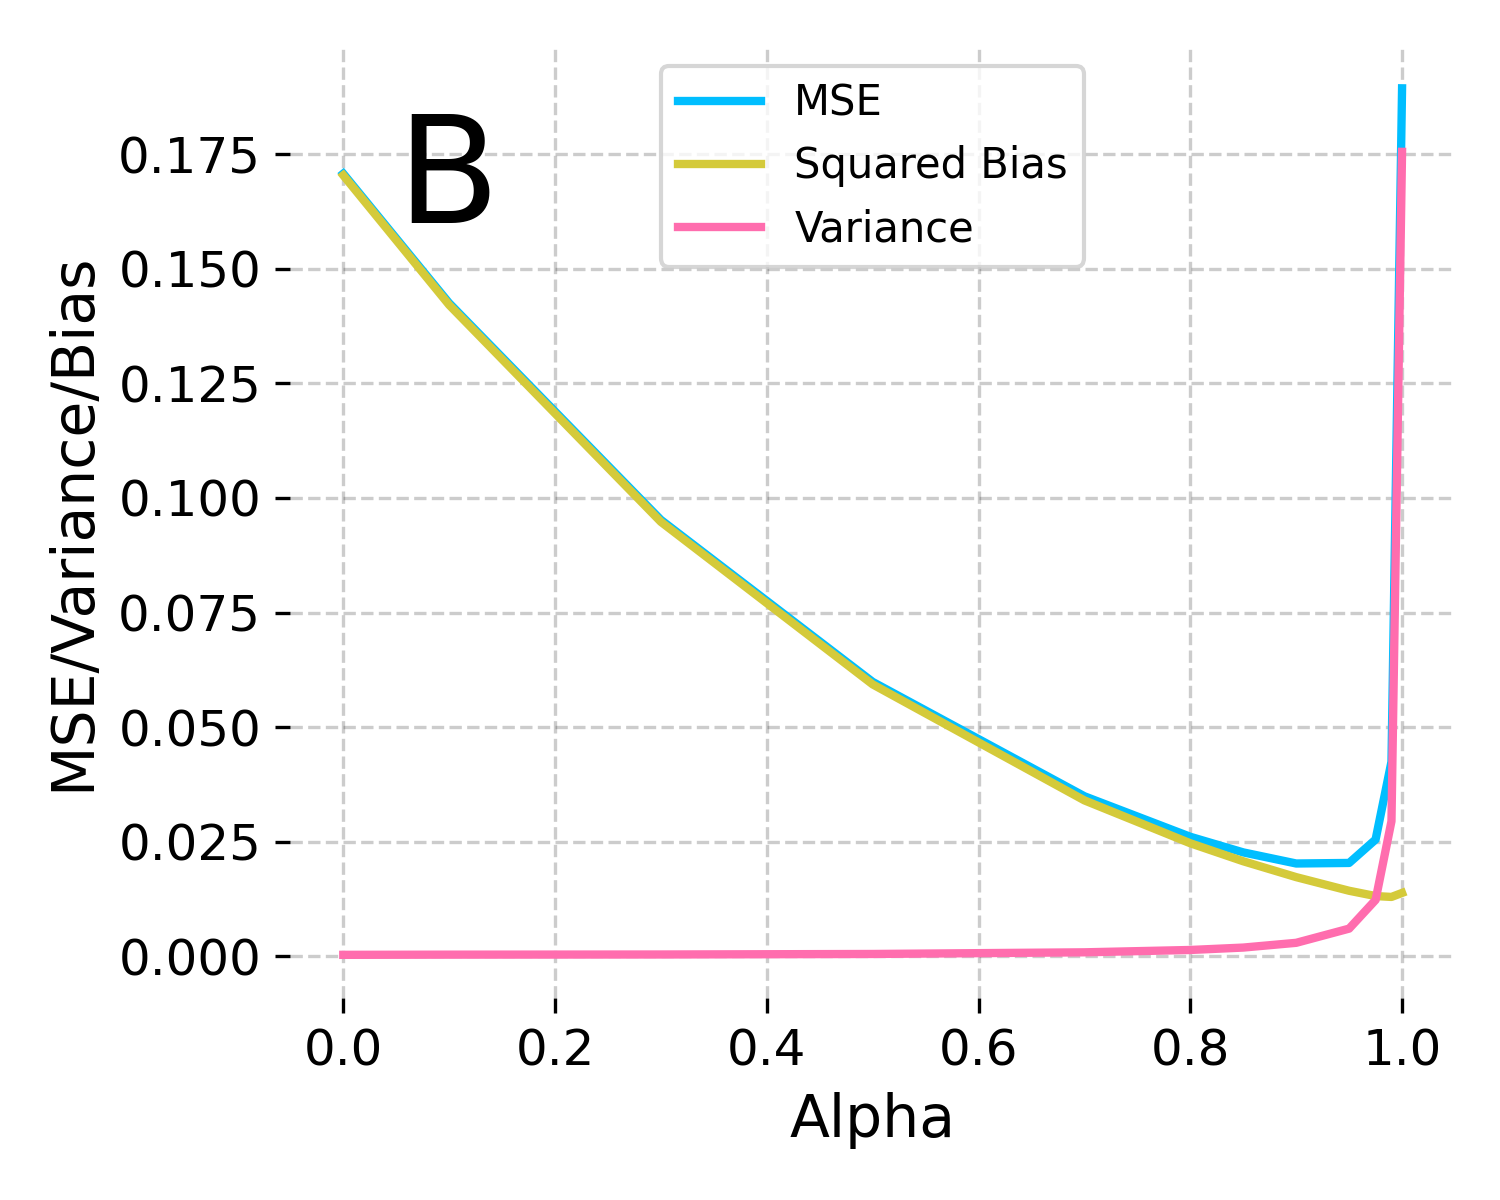
\includegraphics[width=\linewidth]{dmop-biasvar.png}};
\begin{scope}[x={(plot.south east)},y={(plot.north west)}]
% Replace the published labels in their original margins. Curves and ticks are unchanged.
\fill[white] (.018,.20) rectangle (.074,.82);
\node[rotate=90,font=\scriptsize] at (.05,.54) {Score moment};
\fill[white] (.436,.772) rectangle (.78,.953);
\foreach \y/\c in {.917/cyan,.865/gold,.813/pink}{\draw[\c,thick] (.451,\y)--(.502,\y);}
\node[anchor=west,font=\scriptsize,inner sep=0pt] at (.516,.917) {Mean squared norm};
\node[anchor=west,font=\scriptsize,inner sep=0pt] at (.516,.865) {Squared norm of mean};
\node[anchor=west,font=\scriptsize,inner sep=0pt] at (.516,.813) {Variance};
\end{scope}\end{tikzpicture}
\column{.41\textwidth}
1,000 runs of 10,000 particles at the fitted parameters.
\uncover<2->{\gap Variance rises near $\alpha=1$.}
\uncover<3->{\gap The blue curve is the mean squared norm. It equals score MSE at a stationary point.}
\end{columns}
\src{Fig. 1B. Gradient of log likelihood per observation, summed moments across coordinates. Same filter as Fig. 1A.}
\end{frame}

\begin{frame}{Error in the estimated score}
For a fixed dataset $y_{1:N}$, we estimate the score $S=\nabla_\theta\log p_\theta(y_{1:N})$ at $\theta=\phi$.
\pause\gap
$\alpha=1$: $\E\|\widehat S-S\|^2\to0$ as the particle count $J\to\infty$.
\pause\gap
For $\alpha<1$, let $H_N(\alpha)=\sum_{r=0}^{N-1}\alpha^r$. Then
\[
\E\|\widehat S-S\|^2\ \lesssim\
\underbrace{\left[\frac{N(1+\log J)^2}{J}+\frac{N^2}{J^2}\right]H_N(\alpha)^2}_{\text{particle approximation}}
+\underbrace{N^2(1-\alpha)^2}_{\text{discount-bias bound}} .
\]
\src{Theorem 5. After-resampling estimate with multinomial draws, $J\ge2$. Smoothness, bounded positive densities and bounded derivatives (A2, A3, A5), plus sensitivity decay (A6) or joint state--derivative mixing (A6-J).}
\end{frame}

\begin{frame}{Fitting the model}
\begin{center}\begin{tikzpicture}[x=1cm,y=1cm]
\path[use as bounding box] (0,0) rectangle (12,5.4);
\node[obj] (init) at (1.4,3.6) {$\theta_0$};\node[lab] at (1.4,4.7) {Initial fit\\(iterated filtering)};
\node[obj] (theta) at (5.6,3.6) {$\theta_k$};\node[lab] at (5.6,4.7) {Current parameter};
\node (score) at (10,3.6) {$\widehat S_{J,\alpha}(\theta_k)$};
\node[lab] at (10,4.7) {DMOP score};
\draw[arr] (init)--(theta);\draw[arr] (theta)--node[above,lab]{fresh filter}(score);
\node[obj,visible on=<2->] (next) at (5.6,1.1) {$\theta_{k+1}$};
\draw[arr,visible on=<2->] (score.south)|-node[pos=.7,below,lab]{gradient update (Adam)}(next.east);
\draw[arr,visible on=<2->] (next)--(theta);
\node[lab,visible on=<2->] at (2,1.1) {Update baseline\\$\phi\leftarrow\theta_{k+1}$};
\end{tikzpicture}\end{center}
\src{IFAD combines iterated filtering (IF2) with automatic differentiation.}
\end{frame}

\begin{frame}{Likelihood searches for the Dhaka cholera model}
100 parallel searches per method, about 16 minutes per batch.
\begin{columns}[c]
\column{.67\textwidth}\picturefit[5.2cm]{dmop-searches.pdf}
\column{.30\textwidth}
Median log likelihood
\gap
IF2 \hfill $-3754.24$\\
IFAD-$.97$ \hfill $-3744.40$
\end{columns}
\src{IFAD suffix denotes $\alpha$. Red line marks the best fit. Below $-3780$: 2 IF2, 4 IFAD-1, 2 IFAD-0, 0 IFAD-$.97$. Timings exclude diagnostic likelihood calls.}
\end{frame}

\begin{frame}{GPU particle filtering: Dhaka and London}
\begin{center}
Seconds per filter batch\par\medskip
\renewcommand{\arraystretch}{1.35}
\begin{tabular}{lrr}
\toprule
& Dhaka & London \\
\midrule
PyPOMP + CuTe & 3.3 & 10.0 \\
PyPOMP (XLA) & 7.5 & 34.0 \\
pfjax & 11.2 & 1340.3 \\
cuthbert & 11.6 & 1219.6 \\
\bottomrule
\end{tabular}
\end{center}
London: 730 weekly observations, seven daily simulation steps per week.
\src{Warm RTX 3090 timings, float32. $36$ parameter sets $\times$ $36$ replicates, $5{,}000$ particles per filter. Both PyPOMP runs use Threefry. London: PyPOMP uses approximate inverse-CDF draws; pfjax and cuthbert use exact JAX draws. pfjax uses multinomial resampling; the others use systematic resampling.}
\end{frame}
